% article.tex, a sample LaTeX file.
% Run LaTeX on this file twice for proper section numbers.
% A '%' causes LaTeX to ignore remaining text on the line

% Use the following line for draft mode (double spaced, single column)
\documentclass[preprint,pre,floats,aps,amsmath,amssymb]{revtex4}

% Use the following line for journal mode (single spaced, double column)
%\documentclass[twocolumn,pre,floats,aps,amsmath,amssymb]{revtex4}

\usepackage{graphicx}
\usepackage{bm}

\begin{document}

Taken from \url{http://www.physics.csbsju.edu/370/papers/Examples+tex/DC_template/}.
\title{The Scientific Paper: A Template with Tips for Working with \LaTeX}
\author{D.P. Jackson, K. Browne, and J.Q. Student} \affiliation{Department of Physics and Astronomy, Dickinson College, Carlisle, Pennsylvania 17013 USA} \date{\today}

\begin{abstract}
This paper should serve as an outline for writing scientific papers. It contains all of the important sections that should be included in scientific paper as well as descriptions of what should be included in each of these sections. It also contains some useful tips on how to use \LaTeX\ to write scientific papers. The easiest way is to use this document as a template and insert your text and figures as described in the text below. This section is the abstract. The abstract should contain a brief description of the project including relevant description of the problem, data collection procedures, and a summary of results as well as a brief description of how this information fits into the overall field. The abstract may contain equations like $\textbf{E}=\textbf{E}_0\cos (\textbf{k}\cdot\textbf{r}-\omega t+\phi)$ and, as you will notice, inline equations look much better in \LaTeX\ than they do in MS Word. An abstract is usually quite short. Often, the length is limited to between 200 and 400 words.
\end{abstract}

\maketitle

\section{Introduction}
\label{sec:intro}

This paper contains a general outline of the information that should be included in a scientific paper. It provides a good template within which you can easily write a paper. When you start out writing papers, you will likely include most of these sections and utilize this fairly standard format. As you gain experience, you may choose a different ordering or different sections as you find appropriate. Remember this is just a template to help you get started. You will have your own style of writing. Your audience and the content of your paper should be the most important guiding influence when writing any paper. The writing process will go much more smoothly if you take some time to answer a few questions before you begin writing. For example, before you begin writing, ask yourself, ``Who is my audience?'', ``What do I want them to get out of this paper?'', and ``What are the most important ideas to convey with this paper?'' There are lots of other questions you could ask, but these three will help you generate a document that is pitched at the right level and contains information that is useful to your audience.

You should keep in mind that a good scientific paper always introduces the reader to the subject material and provides the appropriate background information that the author thinks the reader will need. A good scientific paper will always make the experimental, computational, or theoretical methods clear enough so that a competent reader should be able to reproduce the work. A clear description of how any data was collected should be included as well as a description of the raw data, generally in graphical format. Any analysis performed on the data should be outlined clearly. Analysis and conclusions drawn from the analysis should generally be described separately from raw data. A paper should end with a set of conclusions based on the analysis.

It is the responsibility of the author to carefully lead the reader from the experimental design through the conclusions tying each piece together. For example, it should be clear to the reader explicitly how your analysis leads from your raw data to your conclusions. If you do not make this clear, no matter whether or not you are right, you have not done your job as an author and will find that you have a hard time convincing anyone that what you have done is valid. Finally, every paper should end with a references section. A scientific paper without any references, indicates that the author believes that every thought conveyed in the paper is original. Any information that you obtain from another source should be cited. The only exception is for material that is considered common knowledge. As a student, your common knowledge will often be somewhat more limited than the average author in a scientific journal. As such, you will often reference information from class notes or textbooks that other authors may not. When in doubt, make a reference. This eliminates any possibility that you will be accused of plagiarism, a very serious transgression indeed.

An introduction generally contains a brief introduction to the material that will be presented. Relevant information includes a clear enunciation of the questions that will be addressed in the paper, background information relevant for understanding the paper, basic theory needed to undersand the contents of the paper, etc.

It is important to take into account your audience when writing the introduction. The purpose of an introduction is most often to give your audience enough information so that they will be able to understand the rest of your paper and put it into a larger context. Depending on your audience, this context may vary. For example, if you are preparing a paper with other physics students in mind as the audience, you will write the introduction so they see how their previous physics knowledge will be useful in understanding this paper. If on the other hand, you are writing this paper for a narrow selection of researchers, you will not need to include as much information. Rather, you will present them with enough information so that they can see how this paper fits in with relevant research.

Because you may not be familiar with \LaTeX, you will undoubtedly have many questions about how to do certain things. This document will serve as a template for producing professional looking papers in \LaTeX. Before you begin to modify this document, make sure you have a copy of it saved somewhere so that you can refer back to it if needed. In addition, there are lots of places to get help with \LaTeX\ (including asking professors in physics and math), but a useful place to begin is to visit http://www.giss.nasa.gov/latex/. All the computers in the physics labs are equipped with a program called TeXshop that runs the \LaTeX\ engine.

If you have any questions about the appropriate style for a scientific paper, you should refer to the American Institute of Physics (AIP) Style Manual at http://www.aip.org/pubservs/style/4thed/toc.html.

\section{Theory}
\label{sec:theory}

Often, if the theory needed to understand a paper is somewhat extensive, a separate section containing a description of the theory will be presented. This section should contain enough theoretical detail to make it possible for a member of your target audience to be able to reproduce any results you come up with. Obviously, the amount of detail that you include will depend on space constraints and the expected level of expertise of your audience.

In the context of a paper written by an undergraduate for a class, you should include all non-obvious steps and be sure to reference material that is not ``common knowledge.'' If you just learned the material in a class, you should include references to where the basic derivation comes from. If you start with a non-trivial expression that you had to look up somewhere, either in a book, a paper, or your notes, you should definitely include a reference.

All equations should be incorporated into the text using a program designed to properly format equations. \LaTeX\ is designed to handle equations, equation numbering, and cross referencing to sections, equations, and figures with ease. In fact, you do not need to worry about numbering any sections or equations, that will be done for you automatically. You may want to refer back to an equation, figure, or section. To do so, you simply label the appropriate item and then refer back to it when needed. For example, to refer back to the introduction, I can type something like ``this is discussed in Sections $\backslash$ref\{sec:intro\} and $\backslash$ref\{sec:theory\}'' to get ``this is discussed in Sections~\ref{sec:intro} and \ref{sec:theory}.'' Notice that I didn't have to worry about the sections numbers. This is a life saver when you are writing a paper with lots of equations and figures. Equation numbering is automatic only in ``displayed math'' mode, which is illustrated here,
\begin{equation}
\textbf{E}=\textbf{E}_0\cos (\textbf{k}\cdot\textbf{r}-\omega t+\phi),
\label{eq:E}
\end{equation}
and here,
\begin{equation}
\textbf{B}=\textbf{B}_0\cos (\textbf{k}\cdot\textbf{r}-\omega t+\phi).
\label{eq:B}
\end{equation}
Of course, I can easily refer back to Eqs.~\ref{eq:E} and \ref{eq:B} without having to remember the numbers.

\section{Experimental Methods}
\label{sec:experiment}

This section is often called experimental design or methods. It contains information about how you went about your experiment. The purpose of this section is to convince your reader that your experimental methods were sound and thorough. That said, if you have made experimental errors that you did not correct, or if you made errors along the way it is your responsibility to report them here. If you do not clearly report your experimental methods, you run the risk of having someone else try your experiment and get other results. This then brings into question the validity of your conclusions and your reputation as a scientist. In addition, if you made errors along the way that you corrected before collecting your final data, it may be worth presenting them here so that others can benefit from your mistakes.

Often you will include a diagram of the experiemtal setup. This is shown in Fig.~\ref{fig:geometry} (note that I didn't have to worry about the figure number). Of course, \LaTeX\ is a typesetting program and is not a graphics program, so you will have to make your graphics in a different program, say, Adobe Illustrator or Xfig. Fortunately, including the figures into a \LaTeX document is a pretty simple matter.

\begin{figure}[ht]
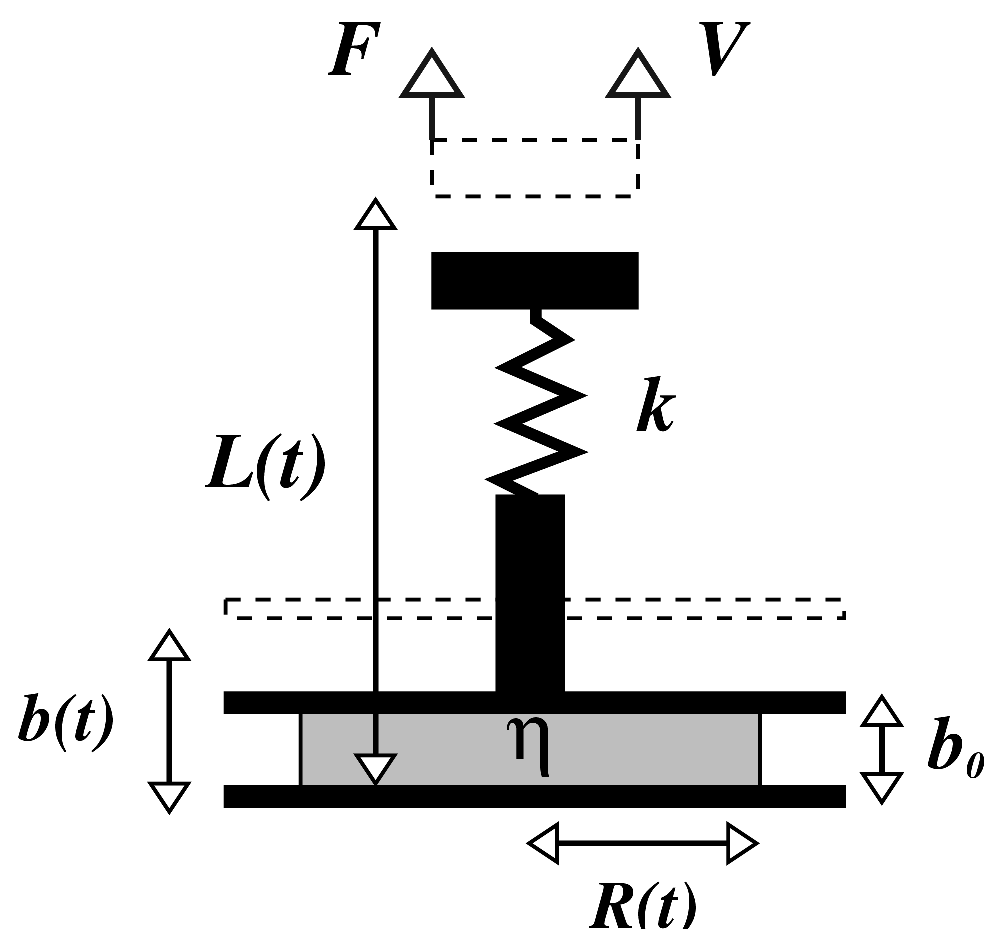
\includegraphics[width=2.8 in]{geometry.eps}
\caption{A sample schematic diagram for an experiment.}
\label{fig:geometry}
\end{figure}

Any diagram you include should contain a fairly detailed figure caption. A good rule of thumb is that if someone reads the abstract and looks at all the figures and captions, they should have a reasonable idea what your paper is about. While this isn?t always possible, it is a good thing to shoot for. That said, this document doesn?t even come close to meeting that requirement, but it also isn?t so much a scientific paper as a how to manual on writing one.

As mentioned before, you should include enough information in your experimental design to make it possible for someone else to reproduce your experiment. You should generally outline what you did with enough detail so that it is clear how you setup your experiment and how you collected your data.

It is particularly important to include anything out of the ordinary. Often we make experimental errors in our setup. It isn't fun, but it happens. If one clearly articulates her setup, it is possible for others to identify these often subtle experimental errors.

\section{Results}
\label{sec:results}

Your paper should contain a section describing your raw results. Often this will be done by including graphs and/or tables of data. This data should generally not be heavily processed. Rather, one should include results in an understandable format that are a good representation of the data obtained by your experiment or computation. You will have a chance to show processed results in the analysis section, but in this section you need to present the reader with your raw data so she can clearly judge the quality of your analysis and conclusions.

Often you have far too much data to include it all. In this case, you will include a sample of raw data with tables or graphs containing straightforward compilations of this data.

It is generally best to make all figures only a single column width, as shown in Fig.~\ref{fig:force}. You generally have three choices of where to place the figures in \LaTeX\. Here (meaning right here if possible), top (meaning top of the page if possible), and bottom (meaning bottom of the page if possible). You may still have to do some fiddling at the end to get them exactly where you want them.
\begin{figure}[ht]
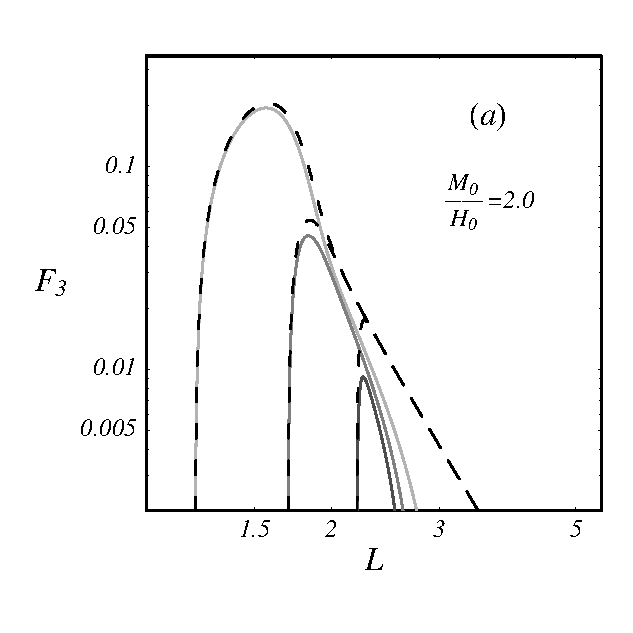
\includegraphics[width=2.8 in]{force.eps}
\caption{Force as a function of length for a particular experiment. The dashed curves represent the nonmagnetic case while the solid curves show the magnetic effects.}
\label{fig:force}
\end{figure}

There are also times when it is appropriate to include a table of data. Unfortunately, tables are not the simplest thing in the world to do in \LaTeX, but they're not all that difficult either. Basically, if you have to make a table, it is best to look for some help in a book or online and then fiddle until you get it looking the way you want. Table~\ref{tab:temps} shows an example of a table that compares two sets of temperature data. As you might expect, simpler tables are easier to make.

\begin{table}[ht]
\caption{Conventional and syringe thermometer readings. The highest and lowest readings were used for calibration.}
\begin{center}
\begin{tabular}{@{\hspace{18pt}} c @{\hspace{18pt}} ||
@{\hspace{12pt}} c @{\hspace{12pt}} | @{\hspace{12pt}} c
@{\hspace{12pt}} }

\hline\hline
Conventional & \multicolumn{2}{c}{Syringe {\hspace{9pt}} } \\ \hline
20$^\circ$C & 1.8cc & 20$^\circ$C \\
27$^\circ$C & 2.4cc & 28$^\circ$C \\
42$^\circ$C & 3.9cc & 46$^\circ$C \\
55$^\circ$C & 5.0cc & 59$^\circ$C \\
67$^\circ$C & 6.0cc & 72$^\circ$C \\
84$^\circ$C & 7.0cc & 84$^\circ$C \\
\hline\hline
\end{tabular}
\end{center}
\label{tab:temps}
\end{table}

In general, you should never include a table in a paper when a figure/graph will do a better job. It is quite rare to see tables in scientific papers. You should never include a long list of data or an excerpt from a spreadsheet unless the particular values in the list are very important. Long lists are hard to read and generally confuse or bore your reader.

Most often tables are used to show a few numbers derived from a larger dataset. This is a good use of tables but should generally occur in the analysis sections because the numbers are derived from the data.

Here is another table. We can reference this table in the same way mentioned in Section 2. Table~\ref{tab:pressure} shows a slightly simpler table.

\begin{table}[ht]
\caption{Force, area, and pressure data for the experiment shown in Fig.~\ref{fig:geometry} and described by Eq.~\ref{eq:B}. Agreement is typically within five percent.}
\begin{center}
\begin{tabular}{l @{\hspace{30pt}} c @{\hspace{18pt}} c}
\hline\hline
& Piston 1 & Piston 2 \\ \hline
Avg. Force (N) & 4.40 & 2.25 \\
Area (cm$^2$) & 6.16 & 2.25 \\
$F/A$ (N/cm$^2$) & 0.714 & 0.717 \\
\hline\hline
\end{tabular}
\end{center}
\label{tab:pressure}
\end{table}

\section{Analysis}
\label{sec:analysis}

After you have clearly described your results, you will describe how you will analyze these results, that is, how you will process the data you collected to obtain information that will help you answer the questions you brought up in the introduction.

It is critically important that the analysis section of a paper is clear. Your job in the analysis section is to convince the reader that the methods you used to get from your results to your conclusions are sound. If your analysis section is incomplete or unclear, your reader may not trust the conclusions you draw.

This is another section where you will often have equations, graphs and tables. Remember that whenever you use an equation, graph or table, it should be referred to in the text. Any equation, graph, figure, or table should fit into your explanations. If you include a graph but make not mention of it in the text, the graph either has not reason to be included, or you have omitted important information from the text.

\section{Conclusion}
\label{sec:conclusion}

Your conclusions section should be brief, but long enough to refocus the reader. The conclusions section describes your assertions based on your data. In essence, it contains the answers you?ve come up with for the questions you asked in the introduction.

You should also make it a point to place your conclusions within a context. That is, you should discuss the possible implications of your conclusions or how they might be relevant to other researchers. This is often hard to do as a student, but not impossible. Some questions you can keep in mind when writing this section are. Why are these conclusions important? Who might these results affect? What could these results be useful for?

It is important to keep in mind that you should not overstate your conclusions. A common error authors make is to over generalize ones conclusions. For example, if I find that a particular type of crystal behaves non-linearly within certain parameters, it is an overgeneralization to conclude that all crystals of that structure will behave the same way. If the author suspects this to be the case, she can state her prediction, but should not assert that it is a fact just because she has a hunch based on her experiment with this one crystal. This leads us to a final sections that you may or may not want to include.

\section{Suggestions for Further Research}
\label{sec:further_research}

This section contains a listing of the directions that the author thinks it will be possible to extend this research. It can be a list of possible future experiments or questions one might ask that are based on the results of the research presented. This section gives the author the opportunity to be somewhat more creative. That said, it should be clear in the paper that the statements made in this sections are suggestions, conjecture and or gut reactions. It is good to include this kind of information, because it helps one to refine her intuition and practice asking interesting scientific questions. Often, this kind of information goes in the conclusion or a section called ``discussion.''

\subsubsection*{Including References}

You must also include a references section in any scientific paper. To omit the references section is to almost certainly commit plagiarism. As mentioned before, you should include references whenever you have used information from another source. This might be a professors notes or a textbook. As you advance in your studies, your references will come more and more from journal articles since these articles generally present more recent results.

In \LaTeX, references are handled very easily in a section called ``thebibliography.'' Thus, you won't actually make a section called references, you will have something called \textit{thebibliography}. All you do is add a ``bibitem'' to \textit{thebibliography} and give it a label. Then, whenever you want to refer to it, you use a $\backslash$cite\{\} command. The order in which you put the items in ``thebibliography'' is the order of the numbering of those items. Therefore, make sure you put these items in the order that they appear in your paper. Here is an example of a book citation~\cite{FHD}, an article citation~\cite{Jackson}, and a comment that might make an important subtle point but one that would detract from the main text~\cite{Comment}.

That is basically all the sections that are normally included in a scientific paper, but there are still some issues that might help you regarding \LaTeX. I have put these into an appendix as an example of how you might use an appendix to put material that is essential to include but inhibits the flow of the paper.

\begin{acknowledgments}

You should always have a short acknowledgements section. This is where you thank people who helped you with the project. These can be people that assisted with construction, people you talked with that gave you good ideas, people you had an email correspondence with, basically anyone that contributed in some way to the success of the project. You would also list fundint agencies in the acknowledgements section.

\end{acknowledgments}

\appendix*

\section{More \LaTeX\ Information}
\label{sec:latex}

This appendix is here to give you a bit more of an introduction to \LaTeX. At this point, it is very short and only includes the most basic items, but I will expand it in the future. If there is something you learned about \LaTeX that was very valuable, please let me know and I will put it in here.

\subsection{Getting Started}

The first thing you have to do is open TeXShop on one of the macs in the lab and then open a tex file (this one, for example). Then you need to typeset the document. Depending on the options in TeXShop, the file will compile and produce a PDF file that you can then read or print out.

\subsection{Fonts}

In a typical scientific paper, you might want to use \textit{italics} or \textbf{bold} fonts occasionally. In \LaTeX, these are accomplished by using the \verb!\textit{}! and \verb!\textbf{}! commands. The text you actually want italicized (or in bold) would be placed inside the curly braces.

\subsection{Math Mode}

In \LaTeX, you enter math mode by typing \verb!$! and then you leave math mode by typing another \verb!$!. Thus, to type an equation, you place it between two dollar signs. For example, typing \verb!$F=ma$! results in $F=ma$. Greek letters are made by typing a backslash and the name of the greek letter. For example, \verb!$\alpha-\beta+\gamma$! results in $\alpha-\beta+\gamma$. Superscripts and subscripts are handled by using \verb!^{}! and \verb!_{}! in math mode respectively. For example, typing \verb!$A_{1}=e^{-x^{2}}$! results in $A_{1}=e^{-x^{2}}$.

So far, all of these examples have been for \textit{inline} equations that occur right in the paragraph you are typing. More often, you will want to put equations on lines all by themselves with an equation number. This is called a displayed equation and is accomplished by using the \textit{equation} environment (an environment in \LaTeX is something that you begin and end such as the \textit{abstract} environment that was used to create the abstract of this document). Thus, to create a displayed equation that has an equation number, you type \verb!\begin{equation}!, then your equation (and a label), then \verb!\end{equation}!. Here is an example:
\begin{equation}
F_m = -\frac{d{\cal E}_m^{(1)} }{db}.
\label{eq:deriv}
\end{equation}
You will have noticed that to make the derivative in Eq.~\ref{eq:deriv}, I had to make a fraction. The fraction command is \verb!\frac{}{}! (in math mode); the numerator goes in the first set of curly braces and the denominator goes in the second set of curly braces. I also used the command \verb!\label{eq:deriv}! in the equation environment so that I can refer to it simply by typing \verb!Eq. \ref{eq:deriv}! to get Eq.~\ref{eq:deriv}.

You may also find the need to write vector equations. There are different methods of writing vectors in a scientific paper. Most textbooks and scientific papers opt to put vectors in bold: $\textbf{F}=m\textbf{a}$. This was accomplished by typing \verb!$\textbf{F}=m\textbf{a}$!. Note that the command \verb!\textbf{}! essentially takes you out of math mode and places a regular boldface letter in the equation. This is traditionally how vectors are written in textbooks with the corresponding magnitudes for $\textbf{F}$ and $\textbf{a}$ written as $F$ and $a$. This works fine except when there is no non-math-mode character to make bold. An example of a math-mode character that does not have a non-math-mode equivalent is $\nabla$, obtained by typing \verb!\nabla!. If you want this as a vector operator and you want it to be bold, you must use the command \verb!\bm! (boldmath) to get $\bm{\nabla}$. This allows you
to write that in general,
\begin{equation}
\bm{\nabla}\times\textbf{A}\ne\bm{\nabla}\cdot\textbf{A}.
\end{equation}
Note the use of \verb!\times! for $\times$, \verb!\cdot! for $\cdot$ and \verb!\ne! for $\ne$. You might also be interested to know that unit vectors can be written using the \verb!\hat{}! command. For example, \verb!\$hat{\textbf{r}}$! results in $\hat{\textbf{r}}$ and \verb!$\hat{\textbf{e}}_{\theta}! results in
$\hat{\textbf{e}}_{\theta}$.

One more quick topic that is sure to be useful is how to break equations. It is quite common to have equations that are too long to fit on a single line. In these instances, you must break the equation into multiple lines. This is done using the \textit{equationarray} environment: \verb!\begin{eqnarray}!$\cdots$\verb!\end{eqnarray}!. In an \textit{equationarray}, each line needs to be separated by \verb!\\! and items surrounded by ampersands (\verb!&!) will be aligned on separate lines. Also, each line will be numbered separately unless you specify\verb!\nonumber! (which is typically what you'll want to do). The following shows an example of a multiline equation:
\begin{eqnarray}
F_{j} &=& \int d {\cal A}\, \Biggl\{ \frac{3\eta \dot{b}}{b^3}
(R^2 - r^2) + [\Psi_j(R) - \Psi_j(r)] \nonumber \\
&\ &\qquad\qquad + \frac{1}{2}\mu_0 \Bigl[ M_{jr}^2(R) -
M_{jz}^2(r) \Bigr] \Biggr\}.
\label{eq:forcej}
\end{eqnarray}
Notice that I have added some space in Eq.~\ref{eq:forcej} to make it look a little nicer. For those that really want to make things look great, fine tuning math equations with a little spacing here and there can really make a difference. In math mode, you can add space with the following commands: \verb!\,! small space, \verb!\:! medium space, \verb!\;! large space, and \verb&\!& negative small space. These can be quite useful in a number of situations. For example, compare \verb!\sqrt{2}x! which gives $\sqrt{2}x$ with \verb!\sqrt{2}\,x! which gives $\sqrt{2}\,x$, or \verb!\int\int dx dy! which gives $\int\int dx dy$ with \verb&\int\!\!\int \!dx\,dy& which gives $\int\!\!\int \!dx\,dy$. The differences are subtle, but for those with a discerning eye, it is wonderful to have such control over your equations. Incidentally, the commands \verb!\quad! and \verb!\qquad! add even larger and larger amounts of space.

Well, that's all for now. I think that about covers the basics. \LaTeX is an extraordinarily powerful program that is capable of probably anything you can imagine. However, it is not always obvious exactly how to accomplish what you want to do. Fortunately, most of the ``basics'' are fairly easy and you should have no problem figuring them out. For more advanced techniques, you may want to consult a book or one of the online manuals (there are lots of them). Have fun and let me know if you need any help!

\begin{thebibliography}{99}
\bibitem{FHD}R. E. Rosensweig, {\it Ferrohydrodynamics} (Cambridge University Press, Cambridge, 1985), and references therein.
\bibitem{Jackson}D. P. Jackson, R. E. Goldstein and A. O. Cebers, Phys. Rev. E {\bf 50}, 298 (1994).
\bibitem{Comment} Here is an example of a comment that you might need to include. This is usually a comment about something very subtle that might be important to include but generally gets in the way of the regular text.
\end{thebibliography}

\end{document}
% End of document.
